%%%%%%%%%%%%%%%%%%%%%%%%%%%%%%%%%%%%%%%%%%%%%%%%%%%%%%%%%%%%%%%%%%%%%%%%%%
%
% Copyright (c) 2007 Jorge Nunes, All Rights Reserved.
%
%%%%%%%%%%%%%%%%%%%%%%%%%%%%%%%%%%%%%%%%%%%%%%%%%%%%%%%%%%%%%%%%%%%%%%%%%%

\documentclass[11pt]{article}

\usepackage[portuges]{babel}
\usepackage[utf8]{inputenc} 
\usepackage{a4}
\usepackage{amsfonts}
\usepackage{float}
\usepackage{graphicx}
\usepackage{subfigure}
\usepackage[colorlinks=true,urlcolor=black,linkcolor=black]{hyperref}

\usepackage{parskip}






\title{Triângulo de Sierpinski}
\author{Jorge Nunes ({\tt\href{mailto:jorgefranconunes@gmail.com}{jorgefranconunes@gmail.com}})}
\date{Agosto 2007}





\begin{document}


\maketitle

O triângulo de Sierpinsky é um fractal no plano dos reais. Na
figura~\ref{fig-triangulo} pode ver-se uma representação do conjunto
dos pontos que formam o triângulo de Sierpinski.

\begin{figure}[H]
  \centering
  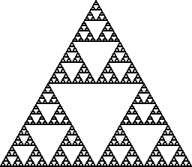
\includegraphics[width=0.3\textwidth]{../images/xxx-007.png}
  \caption{Representação do triângulo de Sierpinski.}
  \label{fig-triangulo}
\end{figure}

Este conjunto é auto-similar. Por auto-similar entende-se que partes
do todo são semelhantes ao todo. Efectivamente, tal como é destacado
na figura~\ref{fig-sierpinski}, o conjunto completo pode ser obtido
através da união de três cópias apropriadamente escaladas e deslocadas
do próprio conjunto.

\begin{figure}[H]
  \centering
  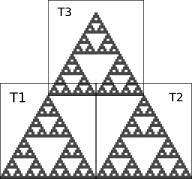
\includegraphics[width=0.3\textwidth]{../images/sierpinski.png}
  \caption{Representação da auto-similaridade do triângulo de Sierpinsky.}
  \label{fig-sierpinski}
\end{figure}
 
Se chamarmos $S$ ao
conjunto dos pontos do triângulo de Sierpinski então podemos dizer que

\[
S = T_1(S) \cup T_2(S) \cup T_3(S)
\]

As funções $T_i : {\mathbb R}^2 \mapsto {\mathbb R}^2$ são
transformações afim que realizam os escalamentos e as translações
específicos para o triângulo de Sierpinski.

Uma transformação afim tem a forma

\[
Tx = Ax + u
\]

onde $A$ é uma aplicação linear (i.~e. corresponde a uma matriz) e o
vector $u$ é uma constante.

No caso do triângulo de Sierpinski as funções $T_i x = A_i x + u_i$
são caracterizadas da seguinte forma:

\[
A_1 = A_2 = A_3 = \left[
  \begin{array}{cc}
    \frac{1}{2} & 0 \\
    0 & \frac{1}{2}
  \end{array} \right]
\]


\[
u_1 = \left[
  \begin{array}{c}
    0 \\
    0
  \end{array}
\right]
\qquad
u_2 = \left[
  \begin{array}{c}
    \frac{1}{2} \\
    0 \end{array}
\right]
\qquad
u_3 = \left[
  \begin{array}{c}
    \frac{1}{4} \\
    \frac{\sqrt{3}}{4}
  \end{array}
\right]
\]


Existem outras formas de definir o triângulo de Sierpinski. Definamos
a função $F : {\mathbb R}^2 \mapsto {\mathbb R}^2$ como

\[
F(\Lambda) = T_1(\Lambda) \cup T_2(\Lambda) \cup T_3(\Lambda)
\]

Então, de acordo com o que tinha atrás já sido exposto temos que o
triângulo de Sierpinsky corresponde ao conjunto dos pontos $S$ onde
$F(S)=S$. Ou seja, o triângulo de Sierpinsky é um ponto fixo da função
$F$.

Mas será que existe mesmo um ponto fixo da função $F$ definida desta
forma? Sim, existe. Haveremos noutro artigo de ver com mais detalhe
como tal pode ser confirmado. Para já fica a ideia de que a sucessão

\[
S_k = F(S_{k-1}), \qquad k \ge 1
\]

converge quando o ponto inicial $S_0$ é um conjunto compacto e desde
que a função $F$ seja uma contração.

Esta forma de definir o triângulo de Sierpinsky tem a vantagem de nos
permitir criar um procedimento para obter uma aproximação desse
conjunto.

As figuras seguintes representam os seis primeiros pontos da sucessão
$S_k$ quando o ponto inicial é o quadrado unitário $S_0 = [0,1] \times
[0,1]$.

\begin{figure}[H]
  \centering

  \subfigure[]{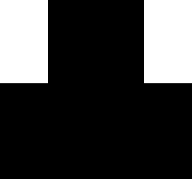
\includegraphics[width=0.3\textwidth]{../images/xxx-001.png}}
  \subfigure[]{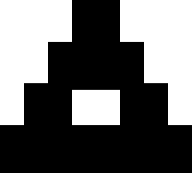
\includegraphics[width=0.3\textwidth]{../images/xxx-002.png}}
  \subfigure[]{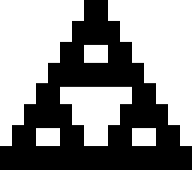
\includegraphics[width=0.3\textwidth]{../images/xxx-003.png}}

  \subfigure[]{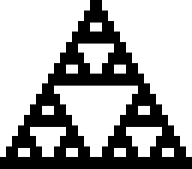
\includegraphics[width=0.3\textwidth]{../images/xxx-004.png}}
  \subfigure[]{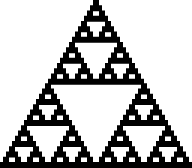
\includegraphics[width=0.3\textwidth]{../images/xxx-005.png}}
  \subfigure[]{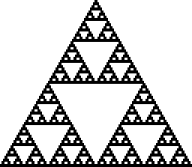
\includegraphics[width=0.3\textwidth]{../images/xxx-006.png}}

  \caption{As seis primeiras iterações da construção to Triângulo de
    Sierpinski.}
\end{figure}

Estas imagens foram geradas utilizando o
\href{http://www.gnu.org/software/octave/}{Octave}. Num futuro artigo
veremos como tal foi conseguido.
  



\end{document}

